\documentclass[aspectratio=169]{beamer}

\usetheme{default}

\usepackage[utf8]{inputenc}
\usepackage[russian]{babel}
\usepackage[OT1]{fontenc}
\usepackage{amsmath}
\usepackage{amsfonts}
\usepackage{amssymb}
\usepackage{graphicx}
\usepackage{etoolbox}
\usepackage{caption}
\usepackage{subcaption}
\captionsetup{compatibility=false}
\usepackage{pifont}
%\usepackage{subfigure}
\usepackage{xcolor}
\usepackage{framed}
\usepackage{empheq}
\usepackage[many]{tcolorbox}
\usepackage{multirow}
\usepackage{tikz}
\usepackage{listings}
\usepackage{tikz}

\definecolor{shadecolor}{cmyk}{0,0,0,1}

\lstset{
	backgroundcolor=\color{lightgray},
	commentstyle=\color{blue},
	frame=single
	breakatwhitespace, 
	language=python, 
	columns=fullflexible, 
	keepspaces, 
	breaklines, 
	tabsize=3, 
	showstringspaces=false, 
	extendedchars=true,
	numbers=left
}

\makeatletter

\setbeamercolor{title}{fg=white}
\setbeamercolor{frametitle}{fg=black}
\setbeamerfont*{title}{family=\sffamily,size=\LARGE}

\setbeamerfont{page number in head/foot}{size=\scriptsize}
\setbeamertemplate{footline}[frame number]
\let\otp\titlepage
\renewcommand{\titlepage}{\otp\addtocounter{framenumber}{-1}}

\setbeamertemplate{background canvas}{%
	\ifnumequal{\c@framenumber}{0}{%
		\vbox to \paperheight{\vfil\hbox to \paperwidth{\hfil
\includegraphics[height=\paperheight]{images/cover.png}\hfil}\vfil}
   }{%
      \ifnumequal{\c@framenumber}{\inserttotalframenumber}{
        \vbox to \paperheight{\vfil\hbox to \paperwidth{\hfil
\includegraphics[height=\paperheight]{images/back.png}\hfil}\vfil}
      }{%
         % Other frames
      }%
   }%
}

\makeatother

\beamertemplatenavigationsymbolsempty

\tcbset{highlight math style={enhanced,colframe=red,colback=white,arc=4pt,boxrule=1pt}}

\usetikzlibrary{shadings,shadows,shapes.arrows}

\newcommand*{\tikzarrow}[2]{%
  \tikz[
    baseline=(A.base),             % Set baseline to the baseline of node content
    font=\footnotesize\sffamily    % Set fontsize of the node content
  ]
  \node[
    single arrow,                  % Shape of the node
    single arrow head extend=5pt,  % Actual width of arrow head
    draw,                          % Draw the node shape
    inner sep=3pt,                 % Separation between node content and node shape
    top color=#1,               % Shading color on top of node
    bottom color=#1,               % Shading color on bottom of node
    % drop shadow                    % Draw a shadow
  ] (A) {#2};%
}

\newcommand{\tikzfancyarrow}[2][2cm]{\tikz[baseline=-0.5ex]\node [arrowstyle=#1] {#2};}
\newcommand*\rot{\rotatebox{90}}

\author{Николай Анохин}
\title{\newline \newline \newline Лекция 3 \\ Алгоритмы кластеризации I}

\begin{document}

\defverbatim[colored]\hier{%
\begin{lstlisting}[tabsize=4,basicstyle=\footnotesize]
function agglomerative(X, K):
	initialize N # number of objects
	initialize C = N # number of clusters
	initialize C_i = x_i # initial clusters
	while C > K:
		C_a = C_b = None # closest clusters
		min_dist = +inf # distance between closest
		for i in 1 .. C:
			for j in i + 1 .. C:
				dist = d(C_i, C_j) # dist. betw. clusters
				if dist < min_dist:
					min_dist = dist
					C_a = C_i
					C_b = C_j		
		merge(C_a, C_b)
		C = C - 1	
	return C_1, ..., C_K
\end{lstlisting}
}

\defverbatim[colored]\swo{%
\begin{lstlisting}[tabsize=4,basicstyle=\footnotesize]
function swo(X, K):
	initialize N # number of objects
	initialize C = N # number of clusters
	initialize C_i = x_i # initial clusters
	while C > K:
		# choose the pair that optimizes 
		# the given criterion J when merged
		C_a, C_b = find_best_merge(J, C_1, ..., C_C) 
		merge(C_a, C_b)
		C = C - 1	
	return C_1, ..., C_K
\end{lstlisting}
}

\defverbatim[colored]\dbscan{%
\begin{lstlisting}[tabsize=4,basicstyle=\ttfamily]
function dbscan(X, eps, min_pts):
	initialize NV = X # not visited objects	
	for x in NV:
		remove(NV, x) # mark as visited
		nbr = neighbours(x, eps) # set of neighbours
		if nbr.size < min_pts:
			mark_as_noise(x)
		else:
			C = new_cluster() 
			expand_cluster(x, nbr, C, eps, min_pts, NV)
			yield C		
\end{lstlisting}
}

\defverbatim[colored]\extc{%
\begin{lstlisting}[tabsize=4,basicstyle=\ttfamily]
function expand_cluster(x, nbr, C, eps, min_pts, NV):
	add(x, C)
	for x1 in nbr:
		if x1 in NV: # object not visited
			remove(NV, x1) # mark as visited
			nbr1 = neighbours(x1, eps)
			if nbr1.size >= min_pts:
				# join sets of neighbours
				merge(nbr, nbr_1) 
		if x1 not in any cluster:
			add(x1, C)				
\end{lstlisting}
}

\defverbatim[colored]\optics{%
\begin{lstlisting}[tabsize=4,basicstyle=\ttfamily]
function optics(X, eps, min_pts)
    for each point x in X
       x.reachability-distance = UNDEFINED
    for each unprocessed point x in X
       N = getNeighbors(x, eps)
       mark x as processed
       output x to the ordered list
       if (core-distance(x, eps, min_pts) != UNDEFINED)
          Seeds = empty priority queue
          update(N, x, Seeds, eps, min_pts)
          for each next z in Seeds
             N' = getNeighbors(z, eps)
             mark z as processed
             output z to the ordered list
             if (core-distance(z, eps, min_pts) != UNDEFINED)
                update(N', z, Seeds, eps, min_pts)
\end{lstlisting}
}

\defverbatim[colored]\update{%
\begin{lstlisting}[tabsize=4,basicstyle=\ttfamily]
function update(N, x, Seeds, eps, min_pts)
    coredist = core-distance(x, eps, min_pts)
    for each z in N
       if (z is not processed)
          new-reach-dist = max(coredist, dist(x, z))
          # z is not in Seeds
          if (z.reachability-distance == UNDEFINED) 
              z.reachability-distance = new-reach-dist
              Seeds.insert(o, new-reach-dist)
          # z in Seeds, check for improvement
          else              
              if (new-reach-dist < z.reachability-distance)
                 z.reachability-distance = new-reach-dist
                 Seeds.move-up(z, new-reach-dist)
\end{lstlisting}
}

\begin{frame}[plain]
\titlepage
\end{frame}

\begin{frame}{Краткое содержание предыдущей лекции}

\vspace{1em}
{\bf Дано.} Признаковые описания $N$ объектов $\mathbf{x} = (x_1, \ldots, x_m) \in \mathcal{X}$, образующие тренировочный набор данных $X$

\vspace{1em}
{\bf Найти.} Модель из семейства параметрических функций 
\[
H = \{h(\mathbf{x, \mathbf{\theta}}): \mathcal{X} \times \Theta \rightarrow \mathcal{Y} \mid \mathcal{Y} = \{1, \ldots, K\}\},
\]
ставящую в соответствие произвольному $\mathbf{x} \in \mathcal{X}$ один из $K$ кластеров так, чтобы объекты внутри одного кластера были похожи, а объекты из разных кластеров различались

\end{frame}

\begin{frame}{Краткое содержание предыдущей лекции}

\begin{enumerate}
\item Смоделировали данные как смесь нормальных распределений
\[
p(\mathbf{x} | \mu_k, \mathbf{\Sigma}_k) = \sum_{k=1}^K \pi_k \mathcal{N}(\mathbf{x} | \mu_k, \mathbf{\Sigma}_k)
\]
\item С применением Maximum Likelihood получили выражения для шагов E и M
\item Предельным переходом получили алгоритм k-means, минимизирующий инерцию
\[
\tilde J(\mu) = \sum_{n=1}^N \sum_{k=1}^K r_{nk} d(\mathbf{x}_n, \mu_k), \quad r_{nk} = \begin{cases}
1, \; \text{для } k = \arg \min_j d(\mathbf{x}_n, \mu_j) \\
0, \; \text{иначе}
\end{cases}
\]
\item Формулируя альтернативные $d(\mathbf{x}_1, \mathbf{x}_2)$ и $J(\mu)$, получили семейство алгоритмов, обучаемых с помощью EM
\end{enumerate}

\end{frame}

\begin{frame}{Нерешенные проблемы}

\begin{figure}
  \begin{subfigure}[b]{.3\linewidth}
    \centering
    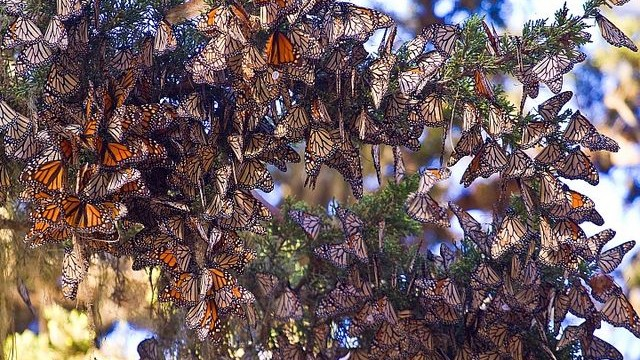
\includegraphics[width=0.9\textwidth]{images/butterflies.jpg}
  \end{subfigure}
  \begin{subfigure}[b]{.3\linewidth}
    \centering
    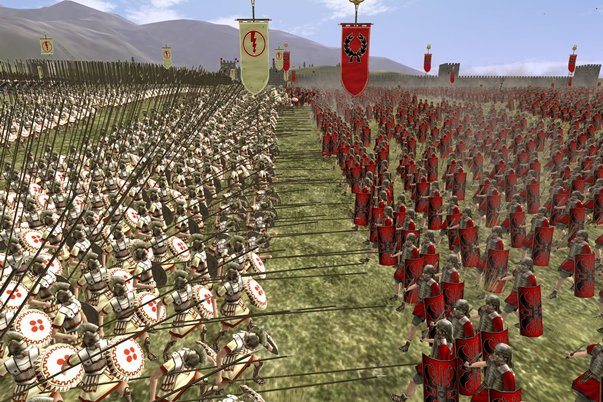
\includegraphics[width=0.75\textwidth]{images/totalwar.jpg}
  \end{subfigure} \quad
  \begin{subfigure}[b]{.3\linewidth} 
    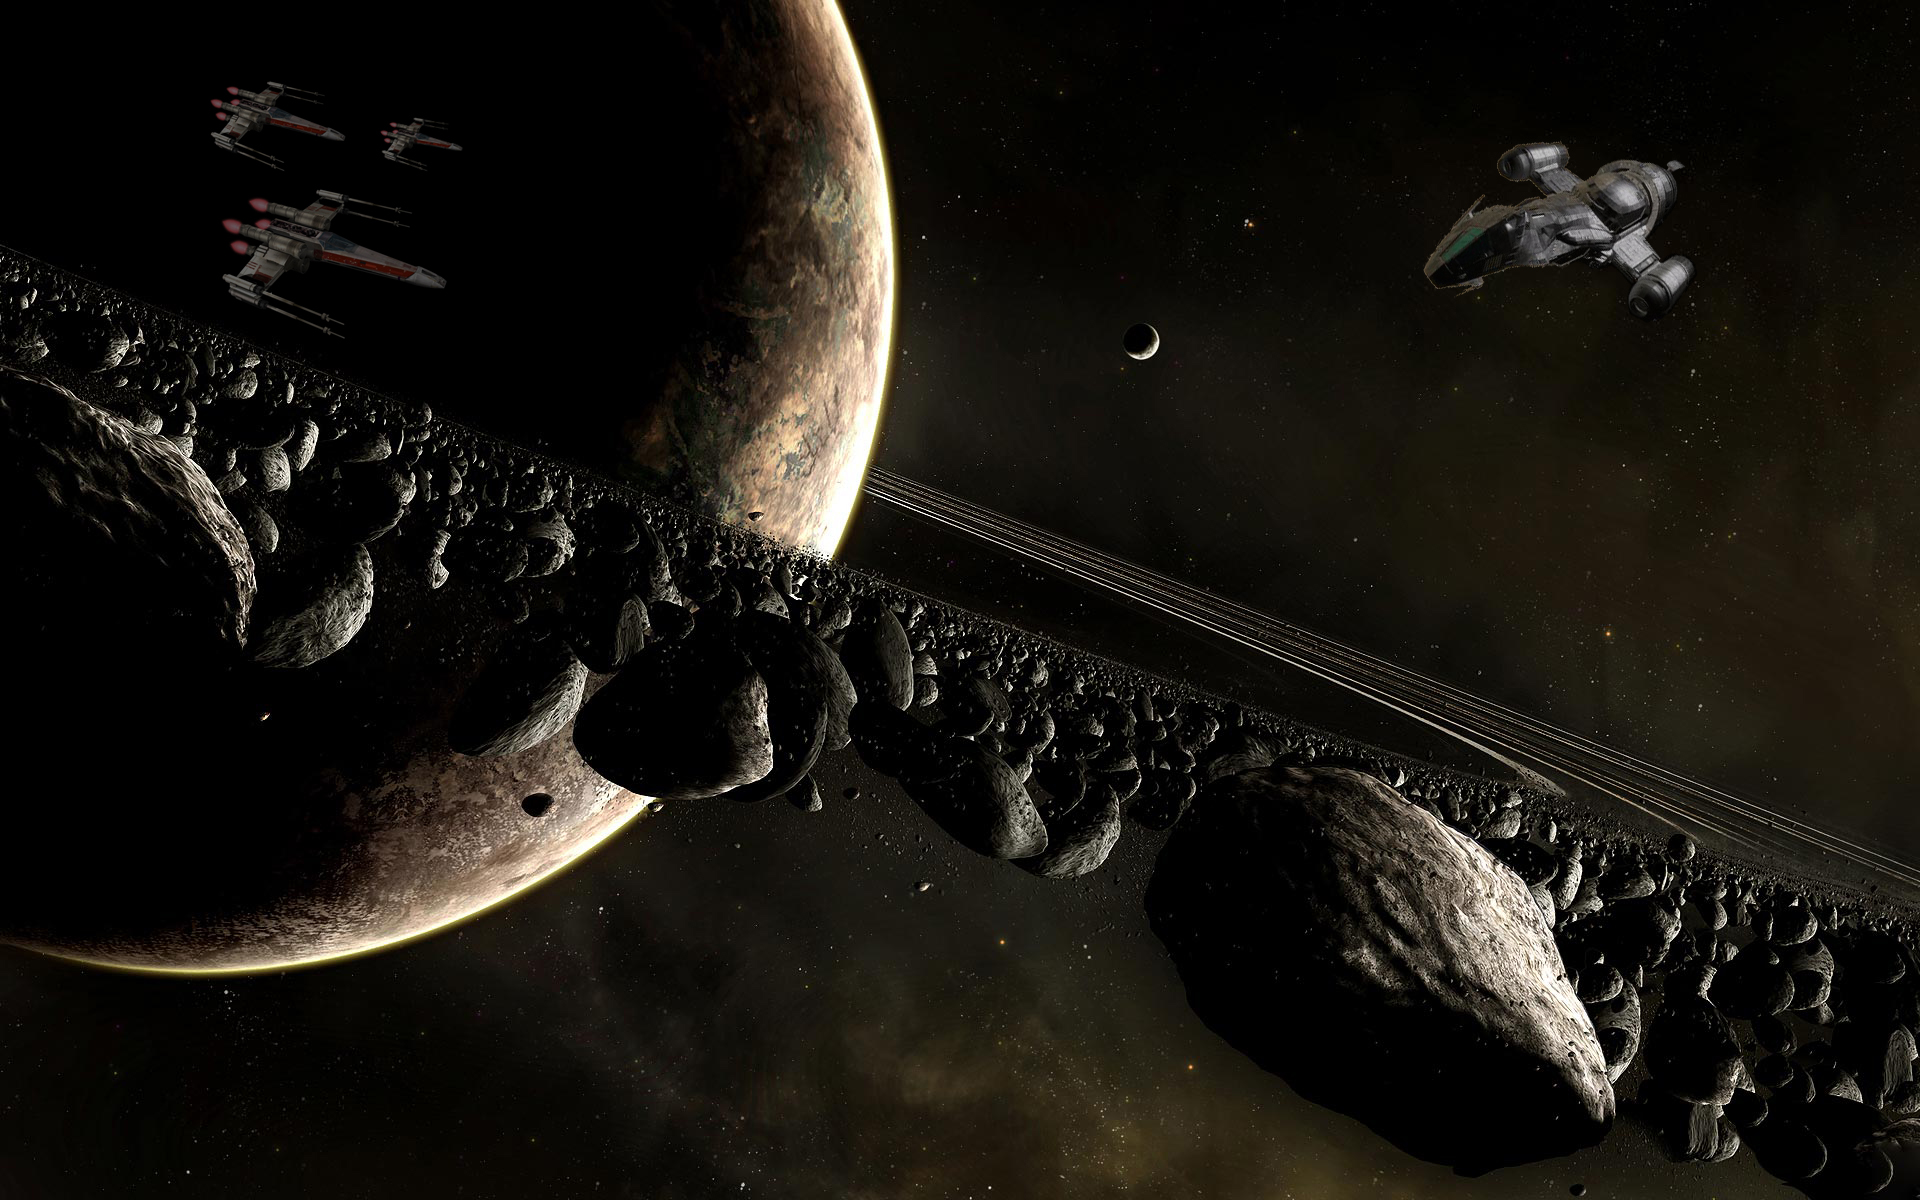
\includegraphics[width=0.8\textwidth]{images/saturn.jpg}
  \end{subfigure}%
\end{figure}

\end{frame}

\begin{frame}

\begin{center}
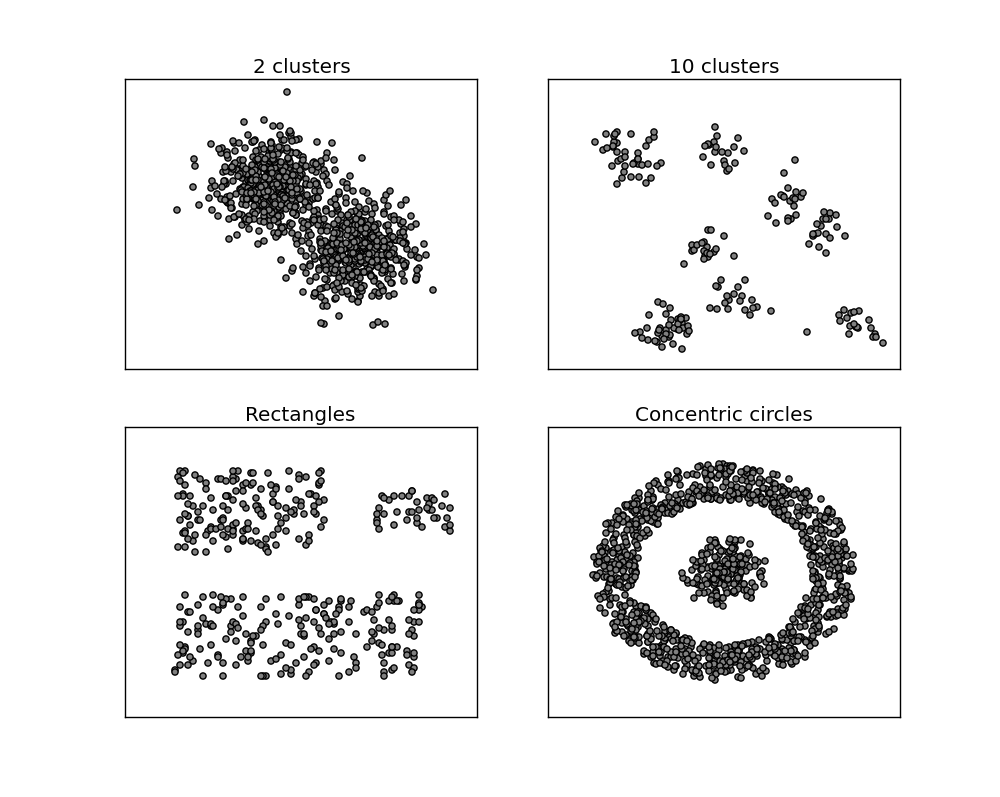
\includegraphics[height=\textheight]{images/datasets.png}
\end{center}

\end{frame}

\begin{frame}

\begin{center}
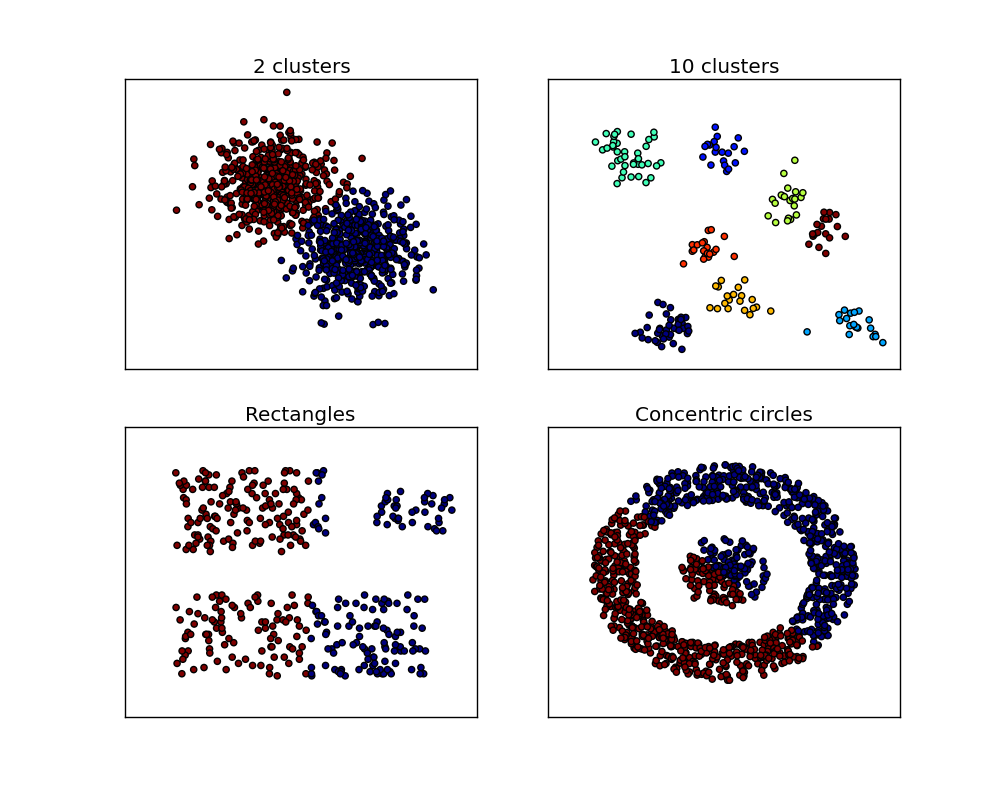
\includegraphics[height=\textheight]{images/datasets_km.png}
\end{center}

\end{frame}

\begin{frame}{План занятия}
\tableofcontents
\end{frame}

% ============================================== %

\section{Функции расстояния}

% ============================================== %

\begin{frame}

\begin{center}
{\Large Функции расстояния}

\vspace{1em}
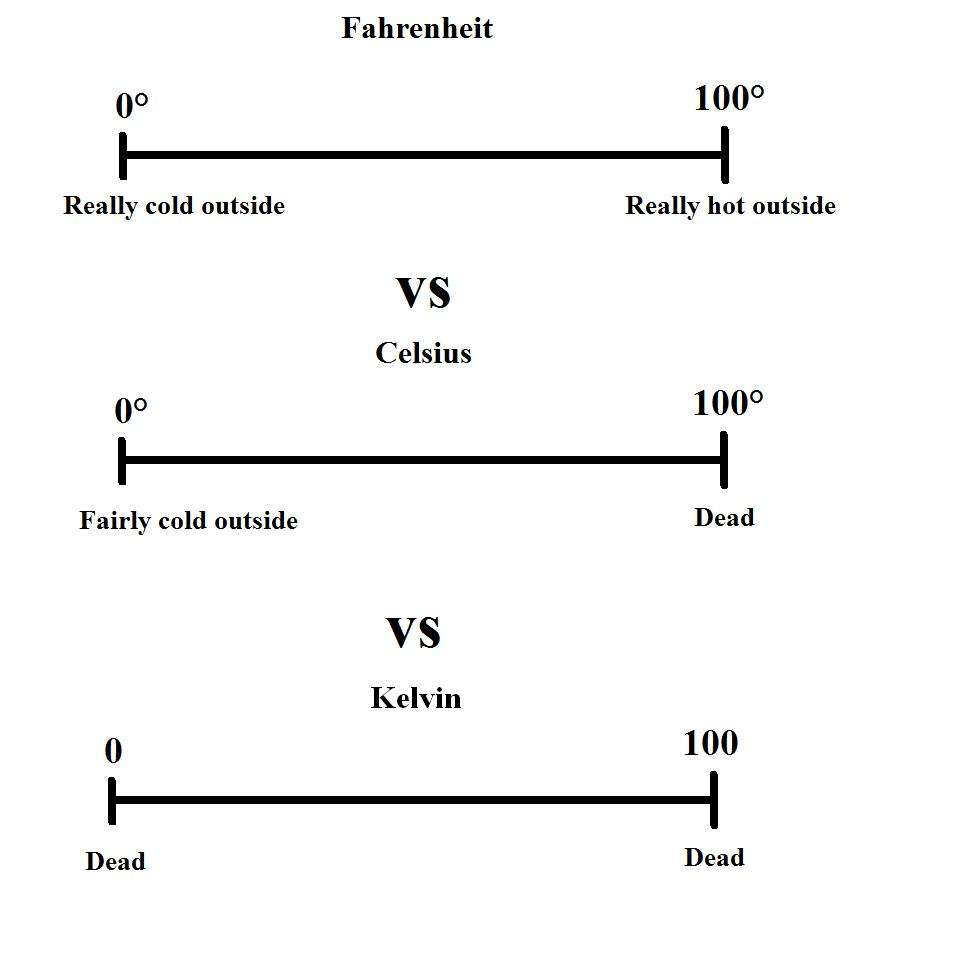
\includegraphics[height=0.8\textheight]{images/celsius.jpg}
\end{center}

\end{frame}

\begin{frame}{Модификации алгоритма}

Взять уже известную нам функцию потерь (инерцию) и ``поиграть'' с функцией расстояния. 
\[
\tilde J(\mu) = \sum_{n=1}^N \sum_{k=1}^K r_{nk} d(\mathbf{x}_n, \mu_k), \quad r_{nk} = \begin{cases}
1, \; \text{для } k = \arg \min_j d(\mathbf{x}_n, \mu_j) \\
0, \; \text{иначе}
\end{cases}
\]
\end{frame}

\begin{frame}{Расстояния 1}

\begin{columns}[T]
    \begin{column}{.5\textwidth}
    \begin{itemize}
		\item Минковского
		\[
		d_r(\mathbf{x}, \mathbf{y}) = \left[ \sum_{j=1}^N |x_j - y_j|^r \right]^{\frac{1}{r}}
		\]
		\item Евклидово $r = 2$
		\[
		d_E(\mathbf{x}, \mathbf{y}) = d_2(\mathbf{x}, \mathbf{y})
		\]
		\item Манхэттэн $r = 1$
		\[
		d_M(\mathbf{x}, \mathbf{y}) = d_1(\mathbf{x}, \mathbf{y})
		\]
		\item $r=\infty$
		\[
		d_\infty(\mathbf{x}, \mathbf{y}) = \max_j |x_j - y_j|
		\]
	\end{itemize}
    \end{column}
       
    \begin{column}{.5\textwidth}
    \vspace{2em}
	\begin{center}
   		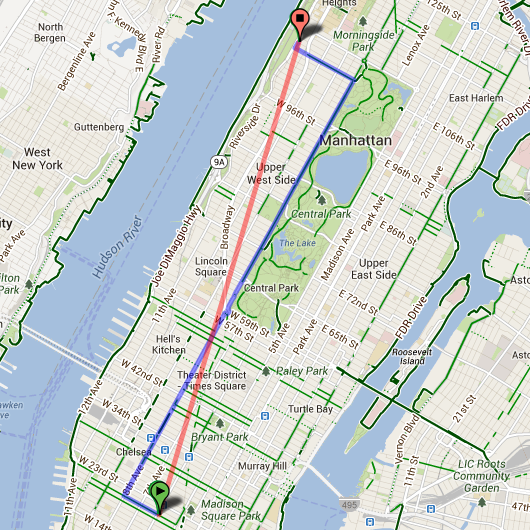
\includegraphics[scale=0.25]{images/manhattan.png}
    \end{center}
    \end{column}
  \end{columns}

\end{frame}

\begin{frame}

\begin{enumerate}
\item Функции расстояния чувствительны к ``масштабу'' данных
\begin{itemize}
\item Преобразовать обучающую выборку так, чтобы  признаки имели нулевое среднее и единичную дисперсию (standartization)
\item Преобразовать обучающую выборку так, чтобы значения признаков лежали на отрезке $[0, 1]$ (normalization)
\end{itemize}
\begin{center}
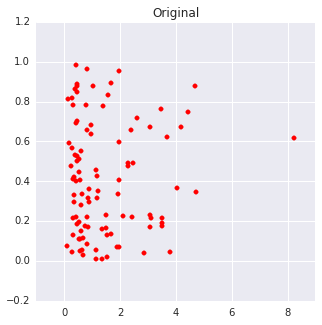
\includegraphics[scale=0.2]{images/orig.png}
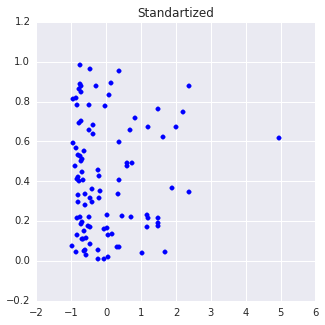
\includegraphics[scale=0.2]{images/std.png}
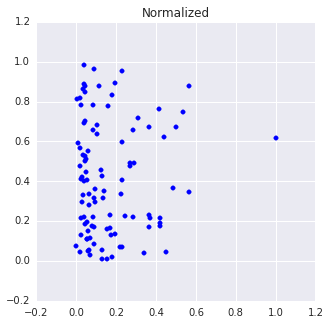
\includegraphics[scale=0.2]{images/norm.png}
\end{center}
\item Есть шанс улучшить качество, применив монотонное преобразование ($\log$, $\sqrt{\;}$)
\begin{center}
$  $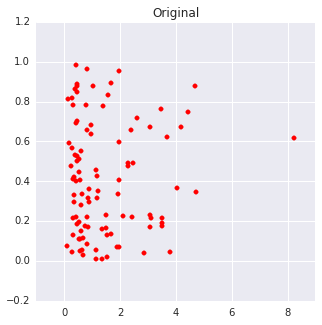
\includegraphics[scale=0.2]{images/orig.png}
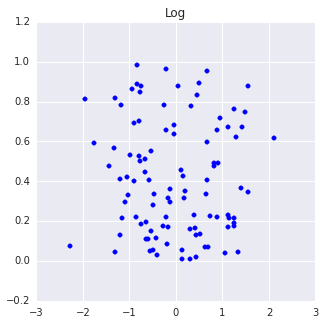
\includegraphics[scale=0.2]{images/log.png}
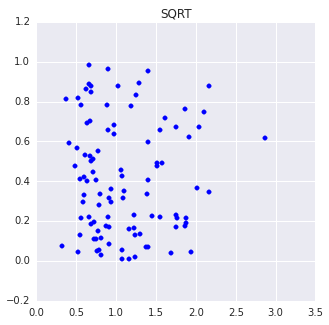
\includegraphics[scale=0.2]{images/sqrt.png}
\end{center}
\end{enumerate}

\end{frame}

\begin{frame}{Расстояния 2}

\begin{columns}[T]

    \begin{column}{.4\textwidth}
    \vspace{5em}
	\begin{center}
   		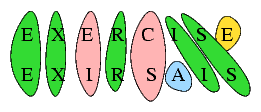
\includegraphics[scale=0.5]{images/edit.png}
    \end{center}
    \end{column}
       
    \begin{column}{.6\textwidth}
    \begin{itemize}
		\item Жаккар
		\[
		d_J(\mathbf{x}, \mathbf{y}) = 1 - \frac{|\mathbf{x} \cap \mathbf{y}|}{|\mathbf{x} \cup \mathbf{y}|}
		\]
		\item Косинус
		\[
		d_c(\mathbf{x}, \mathbf{y}) = \arccos \frac{\mathbf{x} \mathbf{y}}{\|\mathbf{x}\| \|\mathbf{y}\|}
		\]
		\item Правки \\
		{\it $d_e$ -- наименьшее количество удалений и вставок, приводящее $\mathbf{x}$ к $\mathbf{y}$.}
		\item Хэмминг \\
		{\it $d_H$ -- количество различных компонент в $\mathbf{x}$ и $\mathbf{y}$.}
	\end{itemize}
    
    \end{column}
  \end{columns}

\end{frame}

% ============================================== %

\section{Выбор количества кластеров}

% ============================================== %

\begin{frame}

\begin{center}
{\Large Выбор количества кластеров}

\vspace{2em}
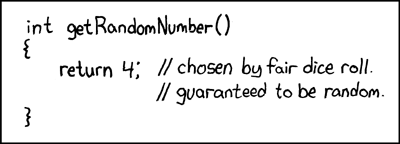
\includegraphics[width=0.7\textwidth]{images/random_number.png}
\end{center}

\end{frame}

\begin{frame}{Выбор наилучшего $K$}

{\it Идея.} Выбрать критерий качества кластеризации и построить его значение для $K = 1, 2, \ldots$

\begin{columns}[]
    \begin{column}{.5\textwidth} 
    \begin{itemize}
	\item средняя сумма квадратов расстояния до центроида
	\item средний диаметр кластера
	\end{itemize} 		    
    \end{column}
    \begin{column}{.5\textwidth}
    \vspace{1em}
    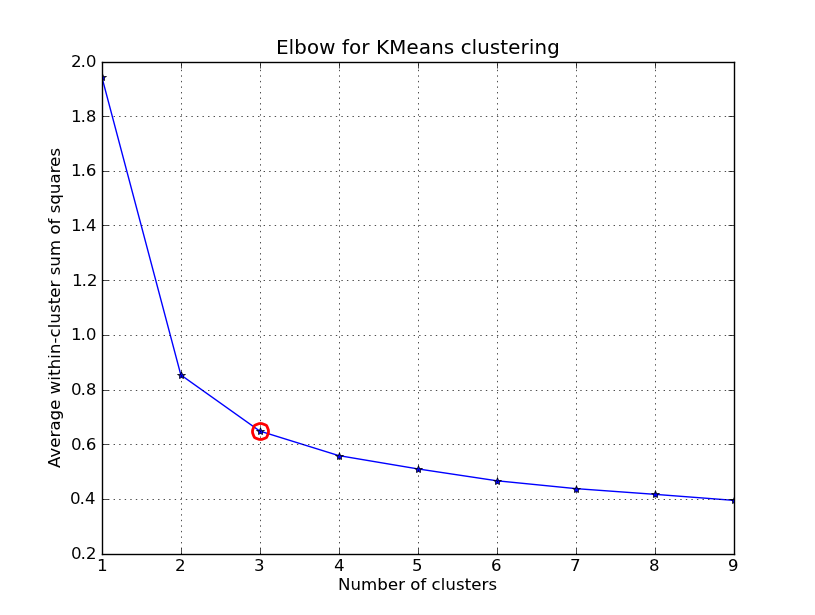
\includegraphics[scale=0.3]{images/elbow.png}    
    \end{column}
\end{columns}

\end{frame}

\begin{frame}{Критерий Silhouette}

Пусть дана кластеризация в $K$ кластеров, и объект $i$ попал в $C_k$

\vspace{1em}
\begin{itemize}
\item $a(i)$ -- среднее расстояние от $i$ объекта до объектов из $C_k$
\item $b(i) = min_{j \neq k} b_j(i)$,  где $b_j(i)$ -- среднее расстояние от $i$ объекта до объектов из $C_j$
\end{itemize}
\[
silhouette(i) = \frac{b(i) - a(i)}{\max(a(i), b(i))}
\]
Средний silhouette для всех точек из $\mathbf{X}$ является критерием качества кластеризации.

\end{frame}

% ============================================== %

\section{Иерархическая кластеризация}

% ============================================== %

\begin{frame}

\begin{center}
{\Large Иерархическая кластеризация\footnote{\href{http://mentalfloss.com/article/59665/feast-your-eyes-beautiful-linguistic-family-tree}{Feast Your Eyes on This Beautiful Linguistic Family Tree}}}

\vspace{1em}
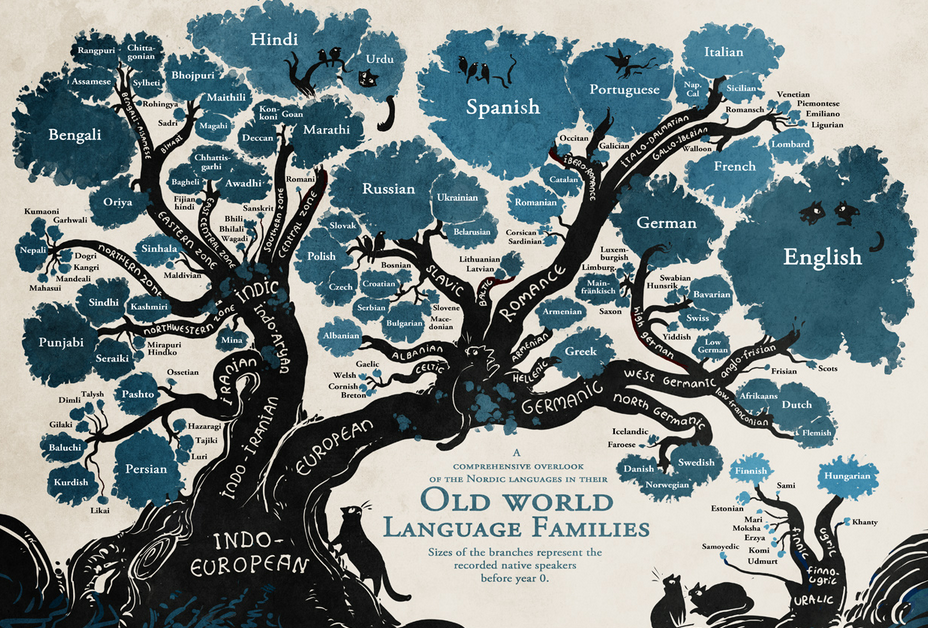
\includegraphics[width=0.95\textheight]{images/languages.png}
\end{center}

\end{frame}

\begin{frame}{Иерархическая кластеризация: идея метода}

{\bf Agglomerative}
\begin{enumerate}
\item начинаем с ситуации, когда каждый объект -- отдельный кластер
\item на каждом шаге совмещаем два наиболее близких кластера
\item останавливаемся, когда получаем требуемое количество или единственный кластер
\end{enumerate}

\vspace{1em}
Divisive
\begin{enumerate}
\item начинаем с ситуации, когда все объекты составляют один кластер
\item на каждом шаге разделяем два один из кластеров пополам
\item останавливаемся, когда получаем требуемое количество или $N$ кластеров
\end{enumerate}

\end{frame}

\begin{frame}{Похожие пернатые динозавры \footnote{\url{http://palaeos.com/vertebrates/coelurosauria/images/feathered_dinosaurs.jpg}}}

\begin{center}
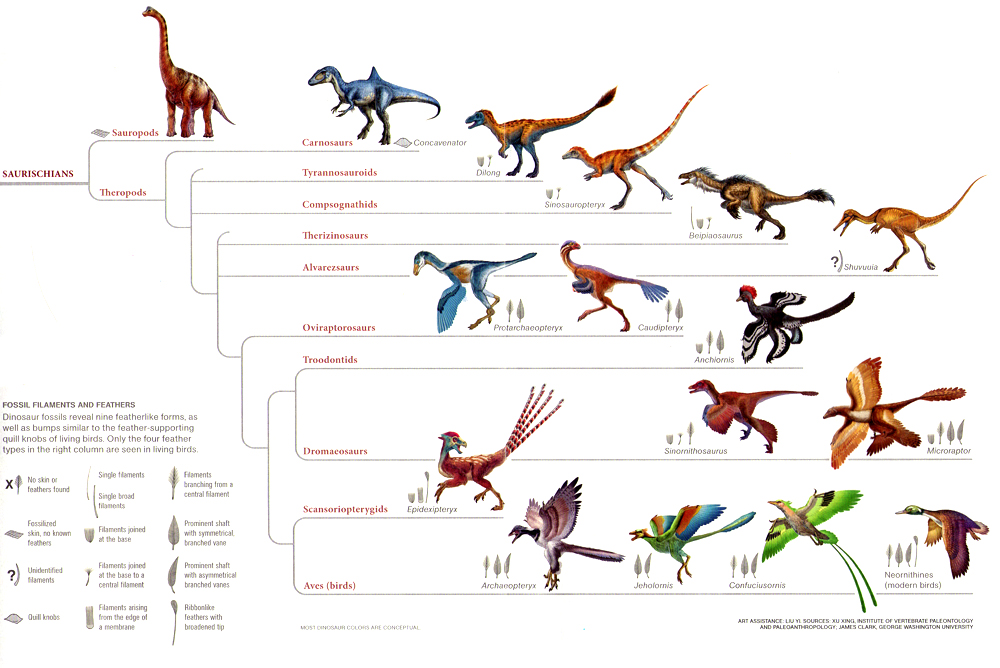
\includegraphics[height=0.8\textheight]{images/dinosaurs.jpg}
\end{center}

\end{frame}

\begin{frame}{Агломеративный алгоритм}

\begin{small}
\hier
\end{small}
память $O(N^2)$, сложность $O(N^2 log N)$

\end{frame}

\begin{frame}{Расстояние между кластерами}

\begin{itemize}
\item single-linkage
\[
d_{min}(C_i, C_j) = \min_{\mathbf{x} \in C_i, \mathbf{x}' \in C_j} \|\mathbf{x} -\mathbf{x}' \|
\]
\item complete-linkage
\[
d_{max}(C_i, C_j) = \max_{\mathbf{x} \in C_i, \mathbf{x}' \in C_j} \|\mathbf{x} -\mathbf{x}' \|
\]
\item average
\[
d_{avg}(C_i, C_j) = \frac{1}{n_i n_j}\sum_{\mathbf{x} \in C_i}\sum_{\mathbf{x}' \in C_j} \|\mathbf{x} -\mathbf{x}' \|
\]
\item mean
\[
d_{mean}(C_i, C_j) = \|\mathbf{m}_i -\mathbf{m}_j \|
\]
\end{itemize}

\end{frame}

\begin{frame}{Задача}

Кластеризовать данные иерархическим методом с использованием расстояний между кластерами $d_{min}$ и $d_{max}$
\begin{center}
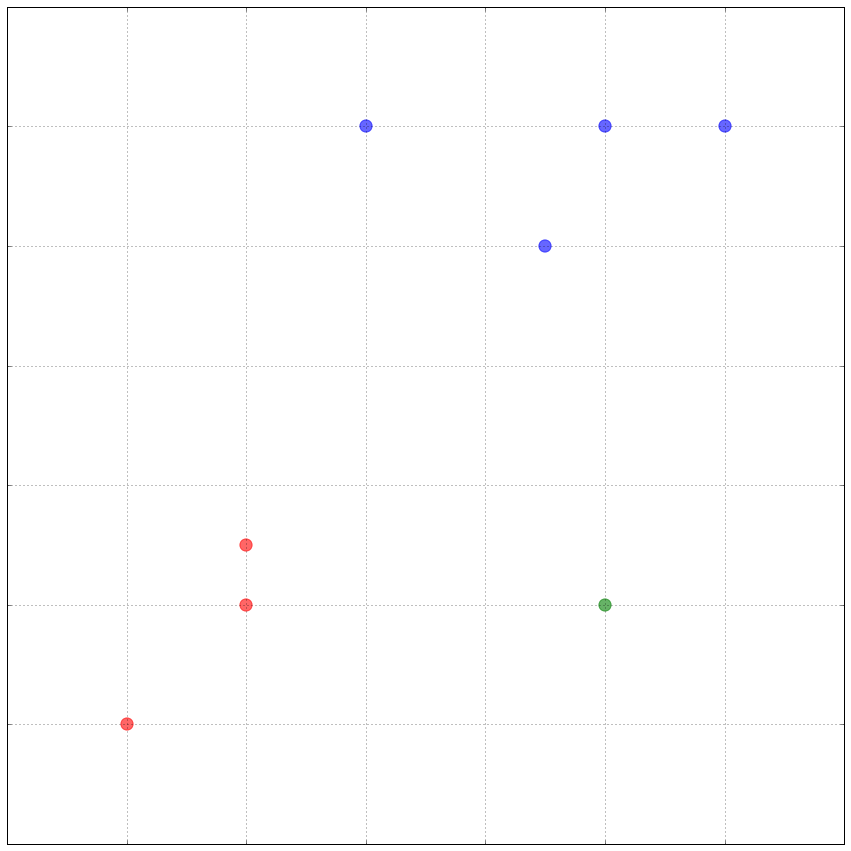
\includegraphics[height=0.7\textheight]{images/toy.png}
\end{center}

\end{frame}

\begin{frame}{Stepwise-optimal HC}

Какой критерий мы оптимизируем?
\swo
$d_{max}$ обеспечивает наименьшее увеличение диаметра кластера \\
$d_e$ обеспечивает наименьшее увеличение квадратичного критерия
\[
d_e(C_i, C_j) = \sqrt{\frac{n_i n_j}{n_i + n_j}} \|\mathbf{m}_i -\mathbf{m}_j \|
\]

\end{frame}

\begin{frame}{Неэвклидовы пространства}

{\it Проблема. } Как измерить расстояние между кластерами, если невозможно определить центроид?

\vspace{1em}
{\it Идея. } В каждом из кластеров выбрать ``типичный'' пример -- clustroid.

\vspace{1em}
Минимизируем
\begin{itemize}
\item сумму расстояний до других объектов в кластере
\item сумму квадратов расстояний до других объектов в кластере
\item максимальное расстояние до других объектов в кластере
\end{itemize}

\end{frame}

\begin{frame}{Пример. Красные и синие штаты\footnote{\url{http://www.wikiwand.com/en/Red_states_and_blue_states}}}

{\color{red} Красные}: Республиканская партия \\
{\color{blue} Синие}: Демократическая партия

\begin{center}
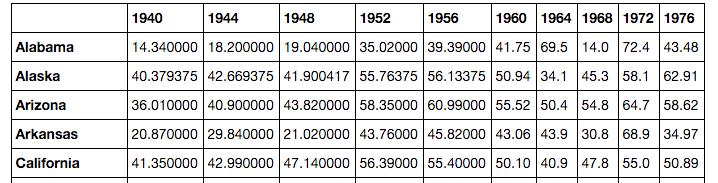
\includegraphics[width=0.8\textwidth]{images/votes.png}
\end{center}

\end{frame}

\begin{frame}{Пример. Красные и синие штаты}

\begin{center}
\begin{figure}
\begin{subfigure}[b]{.45\linewidth}
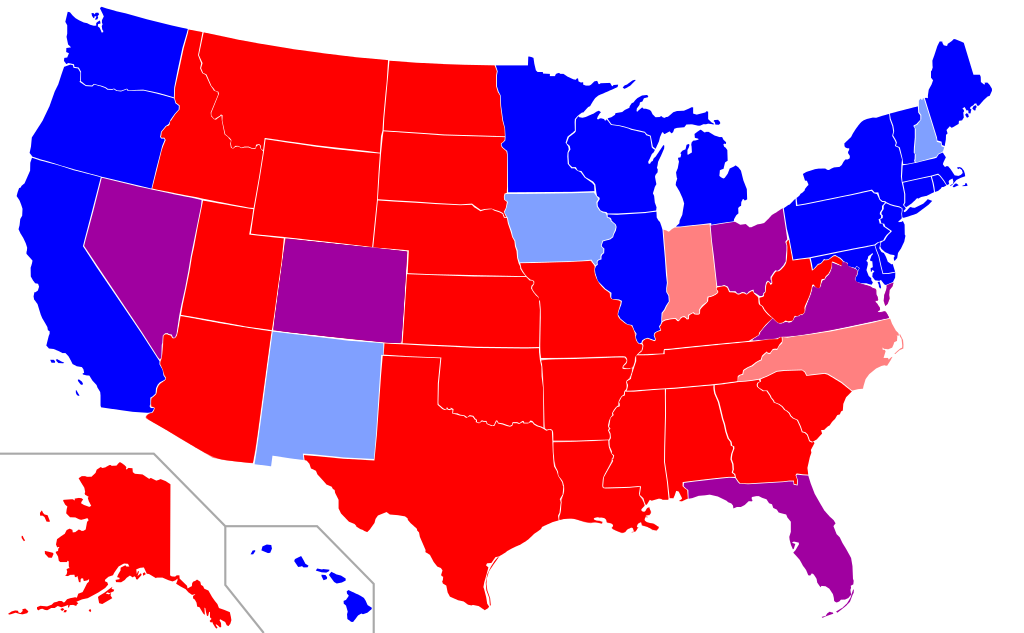
\includegraphics[width=1.0\textwidth]{images/redblue.png}
\caption{Состояние дел на 2012}
\end{subfigure}
\begin{subfigure}[b]{.45\linewidth}
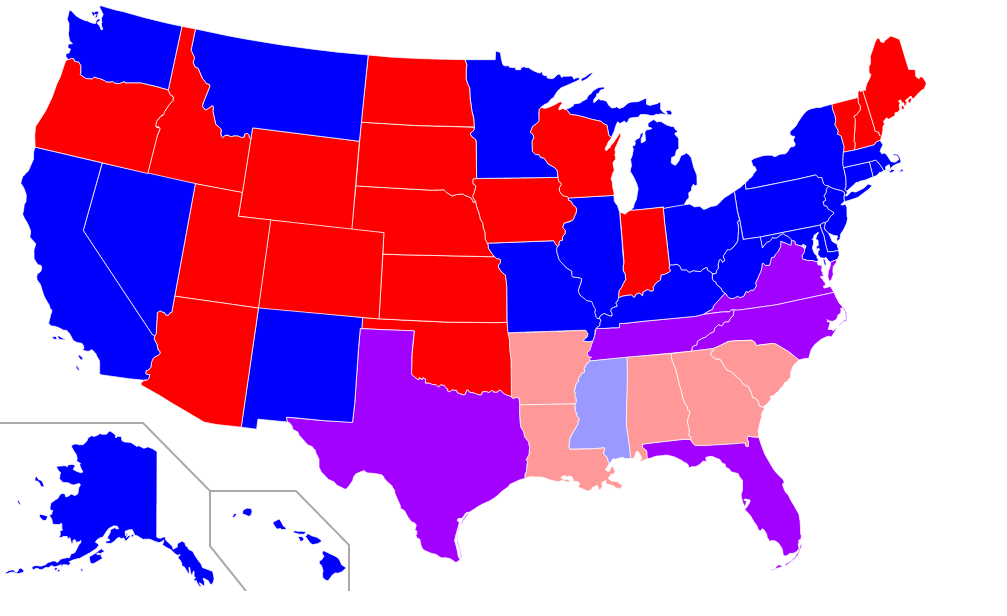
\includegraphics[width=1.0\textwidth]{images/map_hc.png}
\caption{Иер. кл. (euc + avg)}
\end{subfigure}
\end{figure}
\end{center}

\end{frame}

\begin{frame}{Пример. Красные и синие штаты}

\begin{center}
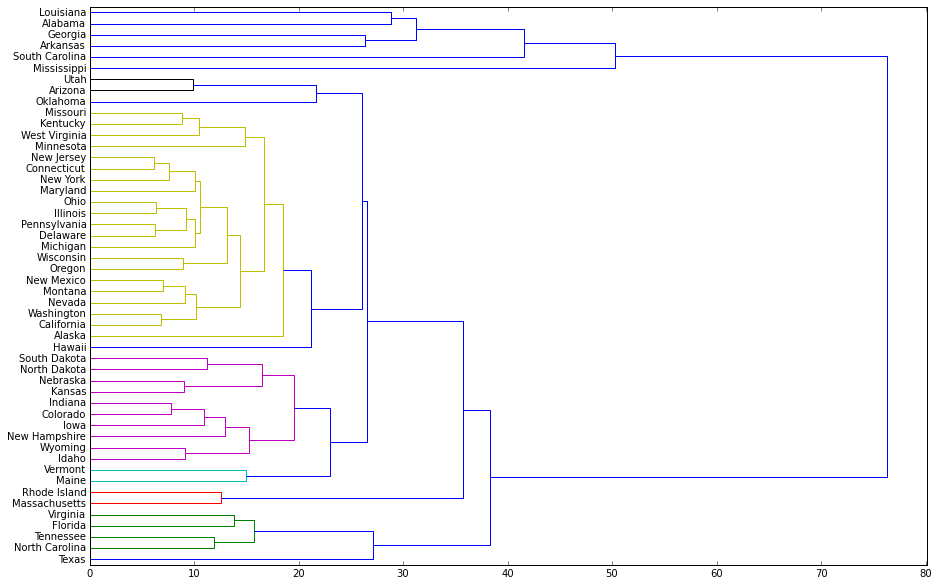
\includegraphics[height=0.9\textheight]{images/states_dendro.png}
\end{center}

\end{frame}

\begin{frame}{Иерархическая кластеризация: итог}

\begin{itemize}
\item[+] Несферические кластеры
\item[+] Разнообразие критериев
\item[+] Любые $K$ из коробки
\item[---] Требует много ресурсов
\end{itemize}

\end{frame}

% ============================================== %

\section{Алгоритмы, основанные на плотности}

% ============================================== %

\begin{frame}

\begin{center}
{\Large Алгоритмы, основанные на плотности}

\vspace{1em}
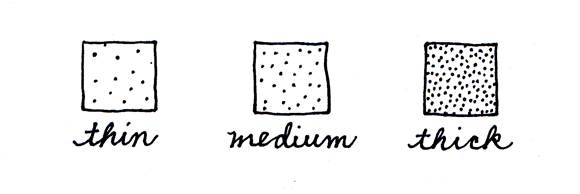
\includegraphics[scale=2.0]{images/density.jpg}
\end{center}

\end{frame}

\begin{frame}{Идея метода\footnote{\url{http://biarri.com/spatial-clustering-in-c-post-2-of-5-running-dbscan/}}}

\begin{itemize}
\item Кластеризация, основанная на плотности объектов
\item Кластеры -- участки высокой плотности, разделенные участками низкой плотности
\end{itemize}

\vspace{1em}
\begin{center}
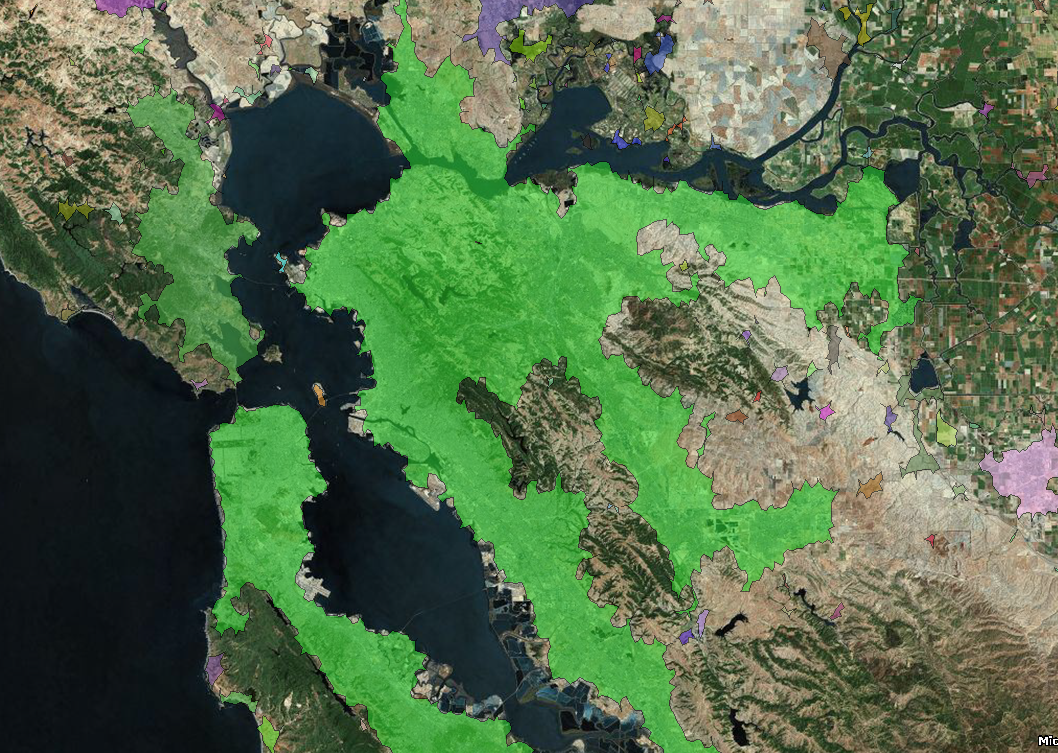
\includegraphics[height=0.4\textheight]{images/dbscan1.png}
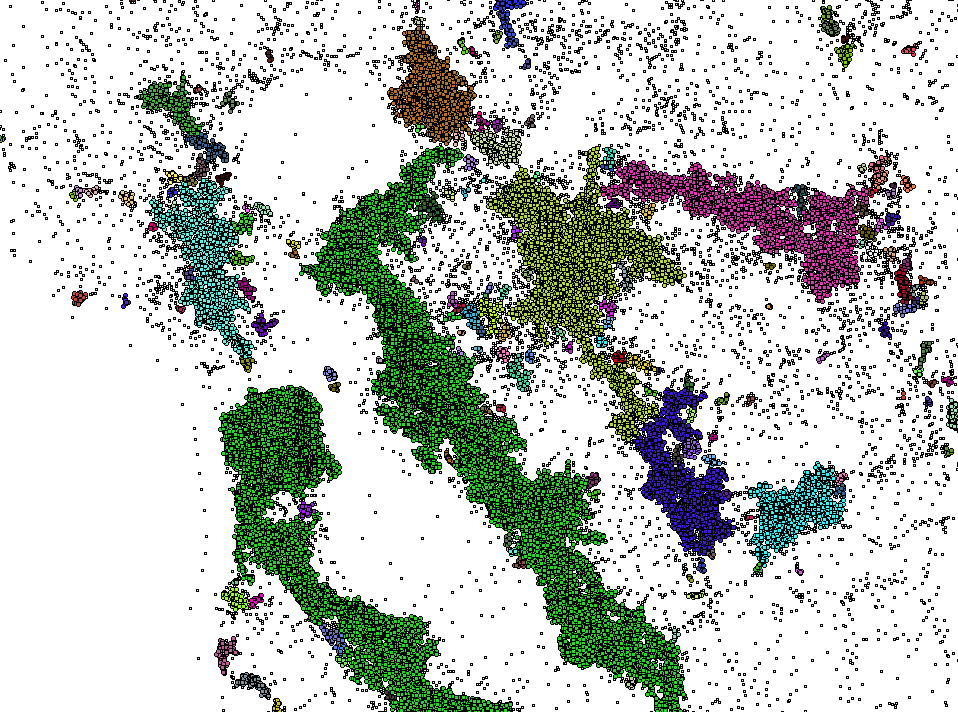
\includegraphics[height=0.4\textheight]{images/dbscan2.png}
\end{center}


\end{frame}

\begin{frame}{Определения}

\begin{block}{Плотность}
Количество объектов внутри сферы заданного радиуса $\varepsilon$
\end{block}

\begin{block}{Core-объект}
Объект $\mathbf{x}$ является core-объектом, если плотность вокруг него больше $min\_pts$
\end{block}

\begin{block}{Граничный-объект}
Объект $\mathbf{x}$ является граничным-объектом, если плотность вокруг него меньше $min\_pts$, но он находится рядом с core-объектом
\end{block}

\begin{block}{Шум}
Объект $\mathbf{x}$ является шумом, если он не является ни core-объектом, ни граничным объектом
\end{block}

\end{frame}

\begin{frame}{Виды объектов}

\begin{center}
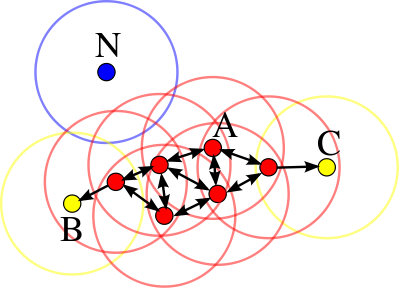
\includegraphics[scale=0.5]{images/points.png}
\end{center}

\end{frame}

\begin{frame}{DBSCAN 1}

\dbscan

\end{frame}

\begin{frame}{DBSCAN 2}

\extc

Сложность: $O(n^2)$ или $O(n \log n)$ ($R^*Tree$) \\ 
Память: $O(n)$ или $O(n^2)$ 

\end{frame}

\begin{frame}{DBSCAN: итог и демо\footnote{\url{http://www.naftaliharris.com/blog/visualizing-dbscan-clustering/}}}

\begin{columns}[]
    \begin{column}{.6\textwidth} 
    \begin{itemize}
	\item[+] не требует $K$
	\item[+] кластеры произвольной формы
	\item[+] учитывает выбросы
	\item[---] Не вполне детерминированный
	\item[---] Не работает при разных плотностях кластеров
	\end{itemize}		    
    \end{column}
    \begin{column}{.4\textwidth}
    \vspace{1em}
    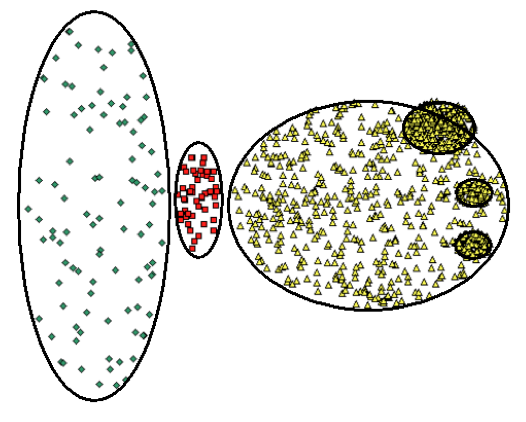
\includegraphics[scale=0.25]{images/dbprob.png}    
    \end{column}
\end{columns}

\end{frame}

\begin{frame}{Задача}

Кластеризовать данные методом DBSCAN
\begin{center}
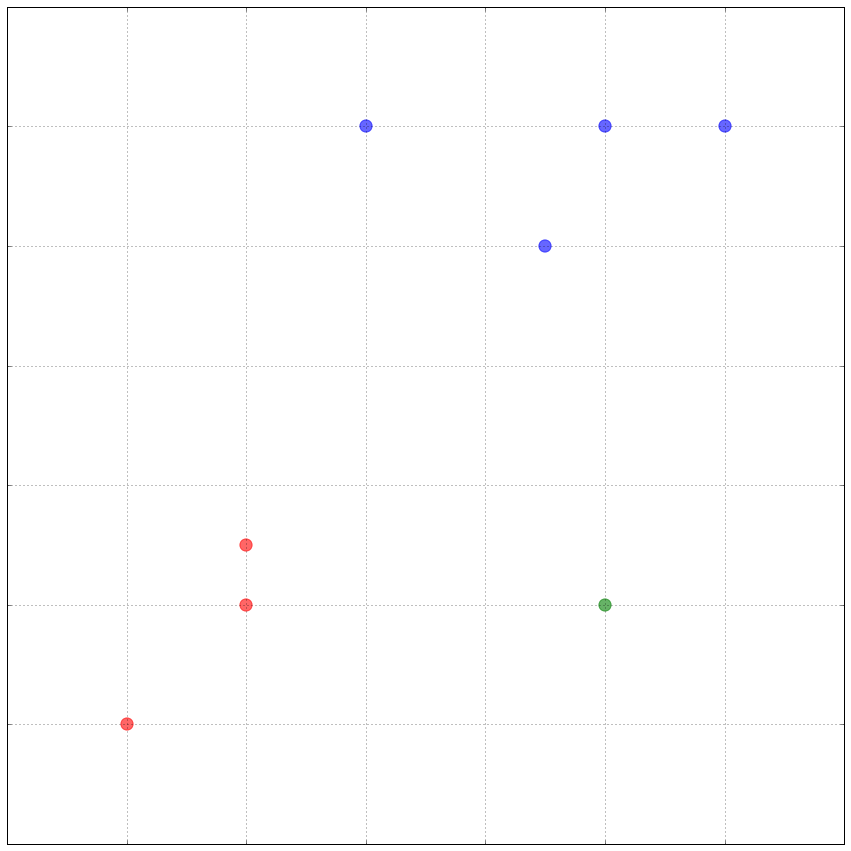
\includegraphics[height=0.7\textheight]{images/toy.png}
\end{center}

\end{frame}

\begin{frame}{OPTICS}
Ordering points to identify the clustering structure

\vspace{2em}
{\it Идея.} не ограничиваться фиксированной плотностью, как в DBSCAN, а варьировать ее в зависимости от того, как много объектов попадают в $\varepsilon$-окрестность.

\vspace{2em}
Пара дополнительных обозначений
\[
\text{core-dist}(p)=\begin{cases}\text{UNDEFINED} & \text{if } |N_\varepsilon(p)| < MinPts\\ MinPts\text{-th smallest distance to } N_\varepsilon(p) & \text{otherwise}\end{cases}
\]
\[
\text{reachability-dist}(o,p) = \begin{cases}\text{UNDEFINED} & \text{if } |N_\varepsilon(p)| < MinPts\\ \max(\text{core-dist}(p), \text{dist}(p,o)) & \text{otherwise}\end{cases}
\]

\end{frame}

\begin{frame}{}

\begin{center}
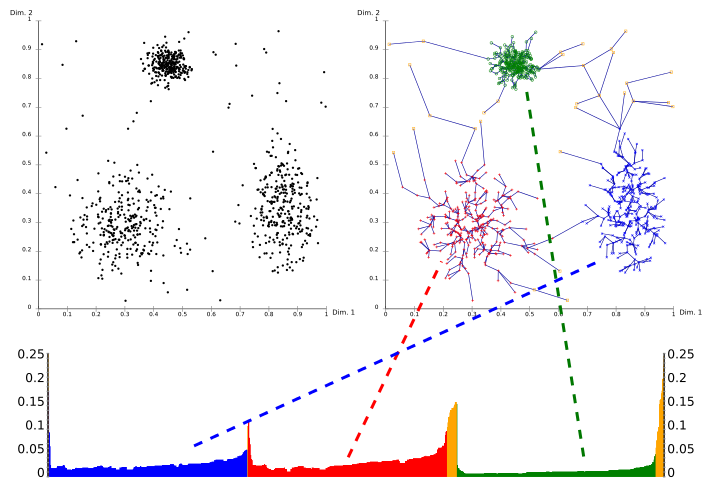
\includegraphics[height=0.9\textheight]{images/optics.png}
\end{center}

\end{frame}

\begin{frame}{OPTICS 1}

\optics

\end{frame}

\begin{frame}{OPTICS 2}

\update

\end{frame}

\begin{frame}{Пример. Красные и синие штаты}

\begin{center}
\begin{figure}
\begin{subfigure}[b]{.45\linewidth}
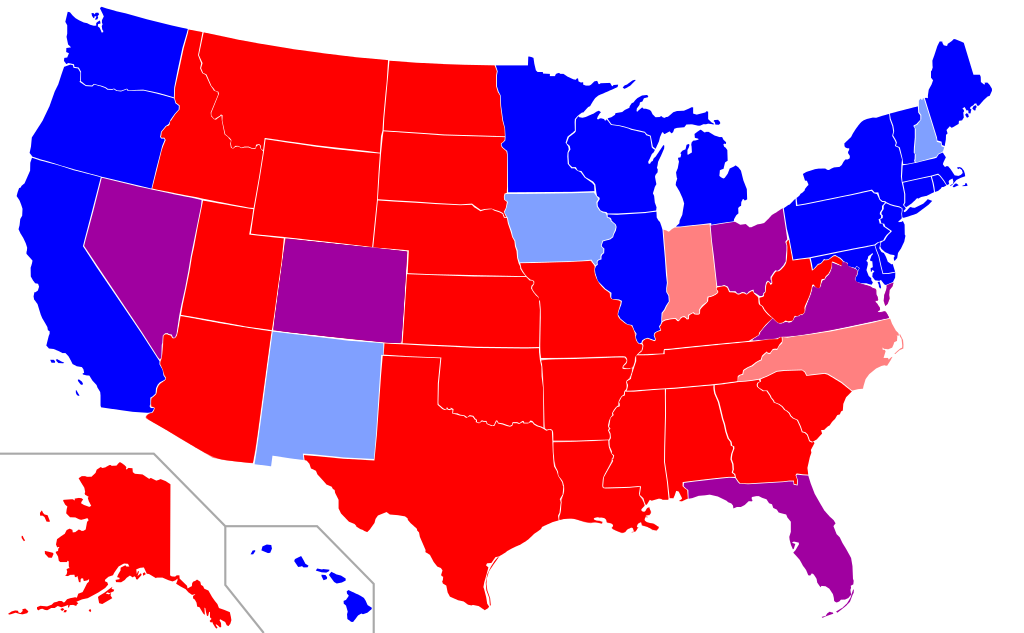
\includegraphics[width=1.0\textwidth]{images/redblue.png}
\caption{Состояние дел на 2012}
\end{subfigure}
\begin{subfigure}[b]{.45\linewidth}
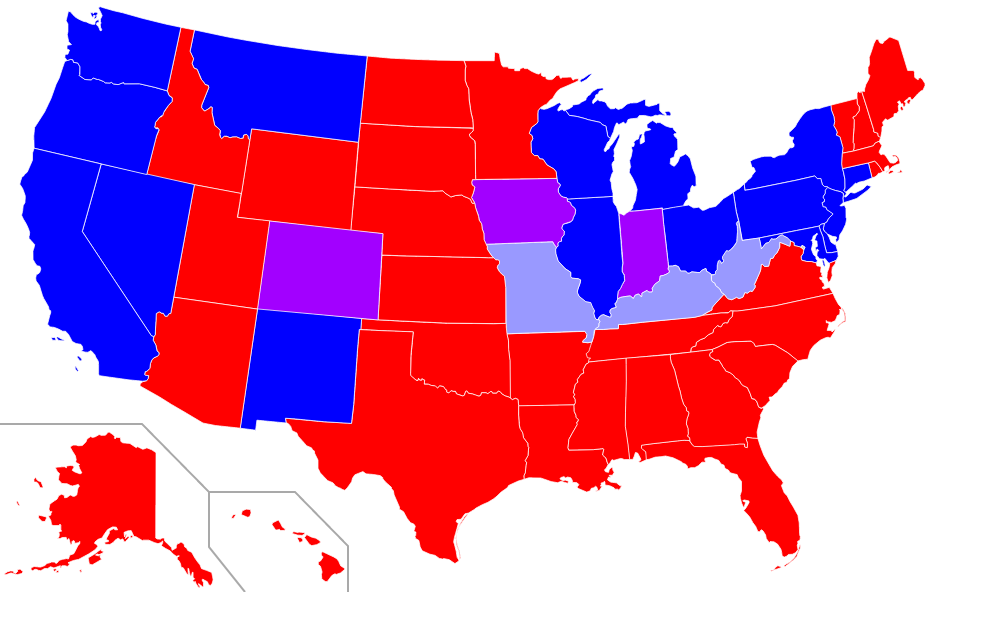
\includegraphics[width=1.0\textwidth]{images/map_db.png}
\caption{DBSCAN}
\end{subfigure}
\end{figure}
\end{center}

\end{frame}

% ============================================== %

\section{Качество кластеризации}

% ============================================== %

\begin{frame}

\begin{center}
{\Large Качество кластеризации}


\includegraphics[scale=0.3]{images/quality.jpg}
\end{center}

\end{frame}

\begin{frame}{Качество кластеризации}

Пусть дана обучающая выборка, для которой правильная кластеризация $C$ известна. С помощью выбранного алгоритма получена кластеризация $K$. Проверить, насколько $K$ совпадает с $C$.

\vspace{1em}
\begin{itemize}
\item Adjusted Rand Index \\
{\it \small
$a$ -- кол-во пар объектов, попавших в один кластер и в $C$, и в $K$ \\
$b$ -- кол-во пар объектов, попавших в разные кластеры и в $C$, и в $K$
\[
RI = \frac{a+b}{C^N_2}, \quad ARI = \frac{RI - E_{rdm}[RI]}{\max(RI) - E_{rdm}[RI]}
\]
}
\item Mutual Information \\
{\it \small
\[
MI = \sum_{c \in C} \sum_{k \in K} p(c, k) \log \frac{p(c, k)}{p(k)p(c)}
\]
}
\end{itemize}

\end{frame}

\begin{frame}[plain]
\begin{center}
{\Large Вопросы}
\end{center}
\end{frame}

\end{document}